\documentclass{article}
% ~ ~ ~ ~ ~ ~ ~ ~ ~ ~ ~ ~ ~ ~ ~ ~ ~ ~ ~ ~ ~ ~ ~ ~ ~ ~ ~ ~ ~ ~ ~ ~ ~ ~ ~ ~ ~ ~ ~ ~ ~ ~ ~ ~ ~ ~ ~ ~

\usepackage[utf8]{inputenc}
\usepackage{amsmath}
\usepackage{amssymb} % for \mathbb
\usepackage{graphicx} % for figures
\usepackage{color}
\usepackage[usenames,dvipsnames]{xcolor}
\usepackage{hyperref} % for hyperlinks
\usepackage{float} % for figures
% ~ ~ ~ ~ ~ ~ ~ ~ ~ ~ ~ ~ ~ ~ ~ ~ ~ ~ ~ ~ ~ ~ ~ ~ ~ ~ ~ ~ ~ ~ ~ ~ ~ ~ ~ ~ ~ ~ ~ ~ ~ ~ ~ ~ ~ ~ ~ ~
% CUSTOM COLOUR
\definecolor{DGrey}{rgb}{0.1,0.1,0.1} % Dark Grey
% ~ ~ ~ ~ ~ ~ ~ ~ ~ ~ ~ ~ ~ ~ ~ ~ ~ ~ ~ ~ ~ ~ ~ ~ ~ ~ ~ ~ ~ ~ ~ ~ ~ ~ ~ ~ ~ ~ ~ ~ ~ ~ ~ ~ ~ ~ ~ ~
\title{ Introduction to Engineering Written Assignment Questions}
\date{January 2013}
\author{Greg Mayer and Daniel Connelly}
% ~ ~ ~ ~ ~ ~ ~ ~ ~ ~ ~ ~ ~ ~ ~ ~ ~ ~ ~ ~ ~ ~ ~ ~ ~ ~ ~ ~ ~ ~ ~ ~ ~ ~ ~ ~ ~ ~ ~ ~ ~ ~ ~ ~ ~ ~ ~ ~
% HEADER/FOOTER
\usepackage{fancyheadings}
\pagestyle{myheadings} % set headings to be user defined
\fancyhead{} % To create custom header, clear default layout
\renewcommand{\subsectionmark}[1]{\markright{{\color{DGrey}\thesubsection} \ {\color{DGrey}#1}}}
\fancyhead[LE,LO]{\subsectionmark} % To create custom header, clear default layout

% ~ ~ ~ ~ ~ ~ ~ ~ ~ ~ ~ ~ ~ ~ ~ ~ ~ ~ ~ ~ ~ ~ ~ ~ ~ ~ ~ ~ ~ ~ ~ ~ ~ ~ ~ ~ ~ ~ ~ ~ ~ ~ ~ ~ ~ ~ ~ ~
% ENUMERATION

\usepackage{enumitem}   % so that question numbers can be formatted 
\setenumerate[1]{label=\thesubsection.\arabic*.} % enumerate environment: add section numbers to items
% ~ ~ ~ ~ ~ ~ ~ ~ ~ ~ ~ ~ ~ ~ ~ ~ ~ ~ ~ ~ ~ ~ ~ ~ ~ ~ ~ ~ ~ ~ ~ ~ ~ ~ ~ ~ ~ ~ ~ ~ ~ ~ ~ ~ ~ ~ ~ ~
% MARGINS
\usepackage{anysize}
\marginsize{2.5cm}{2.5cm}{1cm}{1cm}
% ~ ~ ~ ~ ~ ~ ~ ~ ~ ~ ~ ~ ~ ~ ~ ~ ~ ~ ~ ~ ~ ~ ~ ~ ~ ~ ~ ~ ~ ~ ~ ~ ~ ~ ~ ~ ~ ~ ~ ~ ~ ~ ~ ~ ~ ~ ~ ~
% PAGE NUMBERING
\pagenumbering{arabic}
% ~ ~ ~ ~ ~ ~ ~ ~ ~ ~ ~ ~ ~ ~ ~ ~ ~ ~ ~ ~ ~ ~ ~ ~ ~ ~ ~ ~ ~ ~ ~ ~ ~ ~ ~ ~ ~ ~ ~ ~ ~ ~ ~ ~ ~ ~ ~ ~
% Custom Commands
\newcommand{\Emph}[1]{\textbf{#1}} % Emphasize
\newcommand{\R}{\mathbb{R}} 
\newcommand{\BM}{\begin{bmatrix}} % Begin Matrix
\newcommand{\EM}{\end{bmatrix}} % End Matrix
\newcommand{\BEN}{\begin{enumerate}[leftmargin=1.1cm]}% Begin ENumerate
\newcommand{\EEN}{\end{enumerate}} % End ENumerate
\newcommand{\MB}{\mathbf} % Math Bold

\newcommand{\px}{\frac{\partial}{\partial x}} % Partial wrt x
\newcommand{\py}{\frac{\partial}{\partial y}} % Partial wrt y

\newcommand{\pfx}{\frac{\partial f}{\partial x}} % Partial of f wrt x
\newcommand{\pfy}{\frac{\partial f}{\partial y}} % Partial of f wrt y
\newcommand{\pfxy}{\frac{\partial^2 f}{\partial y \partial x}} % Partial of f wrt y
\newcommand{\pfyx}{\frac{\partial^2 f}{\partial x \partial y}} % Partial of f wrt y

\newcommand{\ux}{\frac{\partial u}{\partial x }} % Partial of u wrt x
\newcommand{\uk}{\frac{\partial u}{\partial k }} % Partial of u wrt k
\newcommand{\ut}{\frac{\partial u}{\partial t}} % Partial of u wrt t
\newcommand{\utt}{\frac{\partial^2u}{\partial t^2}} % Partial of u wrt t
\newcommand{\us}{\frac{\partial u}{\partial s}} % Partial of u wrt t
\newcommand{\uss}{\frac{\partial^2 u}{\partial s^2}} % Partial of u wrt t
\newcommand{\kx}{\frac{\partial k}{\partial x }} % Partial of k wrt x
\newcommand{\kt}{\frac{\partial k}{\partial t }} % Partial of k wrt t

\newcommand{\pxu}{\frac{\partial x}{\partial u}} % x wrt u
\newcommand{\pxv}{\frac{\partial x}{\partial v}} % x wrt v
\newcommand{\pxw}{\frac{\partial x}{\partial w}} % x wrt v
\newcommand{\pxt}{\frac{\partial x}{\partial t}} % x wrt t
\newcommand{\pyu}{\frac{\partial y}{\partial u}} % y wrt u
\newcommand{\pyv}{\frac{\partial y}{\partial v}} % y wrt v
\newcommand{\pyw}{\frac{\partial y}{\partial w}} % y wrt v
\newcommand{\pyt}{\frac{\partial y}{\partial t}} % y wrt t
\newcommand{\pzu}{\frac{\partial z}{\partial u}} % z wrt u
\newcommand{\pzv}{\frac{\partial z}{\partial v}} % z wrt v
\newcommand{\pzw}{\frac{\partial z}{\partial w}} % z wrt v
\newcommand{\pzt}{\frac{\partial z}{\partial t}} % z wrt t


\newcommand{\VCT}{\textit{Vector Calculus} by Michael Corral} % Vector Calculus Textbook
\newcommand{\CAT}{\textit{College Algebra} by Carl Stitz and Jeff Zeager} % College Algebra Textbook
\newcommand{\From}{The following questions are related to } % Questions ....
% ~ ~ ~ ~ ~ ~ ~ ~ ~ ~ ~ ~ ~ ~ ~ ~ ~ ~ ~ ~ ~ ~ ~ ~ ~ ~ ~ ~ ~ ~ ~ ~ ~ ~ ~ ~ ~ ~ ~ ~ ~ ~ ~ ~ ~ ~ ~ ~
% ONLY USED FOR EDITING
\newcommand{\rednote}[1]{{\color{red}\textit{\textbf{#1}}}} % Shortcut for formatting notes for developers
\newcommand{\FromC}[1]{{\color{DGrey}\textit{#1}}} % Shortcut for coloring the "from" text
% ~ ~ ~ ~ ~ ~ ~ ~ ~ ~ ~ ~ ~ ~ ~ ~ ~ ~ ~ ~ ~ ~ ~ ~ ~ ~ ~ ~ ~ ~ ~ ~ ~ ~ ~ ~ ~ ~ ~ ~ ~ ~ ~ ~ ~ ~ ~ ~
% AUGMENTED MATRIX MACRO
% thanks to http://tex.stackexchange.com/questions/2233/whats-the-best-way-make-an-augmented-coefficient-matrix
\newenvironment{amatrix}[1]{%
  \left[\begin{array}{@{}*{#1}{c}|c@{}}
}{%
  \end{array}\right]
}
% ~ ~ ~ ~ ~ ~ ~ ~ ~ ~ ~ ~ ~ ~ ~ ~ ~ ~ ~ ~ ~ ~ ~ ~ ~ ~ ~ ~ ~ ~ ~ ~ ~ ~ ~ ~ ~ ~ ~ ~ ~ ~ ~ ~ ~ ~ ~ ~
% PAGE LAYOUT
\addtolength{\topmargin}{10pt}
\addtolength{\headsep}{10pt}
\addtolength{\textheight}{-20pt}



\setenumerate[1]{label=\arabic*.} 

\date{}
% ~ ~ ~ ~ ~ ~ ~ ~ ~ ~ ~ ~ ~ ~ ~ ~ ~ ~ ~ ~ ~ ~ ~ ~ ~ ~ ~ ~ ~ ~ ~ ~ ~ ~ ~ ~ ~ ~ ~ ~ ~ ~ ~ ~ ~ ~ ~ ~
\begin{document}
\begin{center}
\textsc{\LARGE Final Exam}\\[0.5cm]
\end{center}
\section*{Questions}

\begin{enumerate}
% ~~~~~~~~~~~~~~~~~~~~~~~~~~~~~~~~~~~~~~~~~~~~~~~~~~~~~~~~~~~~~~~~~~~~~~~~~~~~~~~~~
\item % TRAFFIC FLOW
The diagram below shows the typical flow of traffic (in number of vehicles per hour) on a Saturday afternoon in the downtown area of a city where all the streets are one-way streets. For example, at the intersection of Main St. and North Ave., the number of vehicles that flow into the intersection per hour is typically 400 + 200, and the number of cars that flow out of that intersection is $x_1+x_2$. 
\begin{figure}[H]
  \vspace{-5pt}
  \begin{center}
    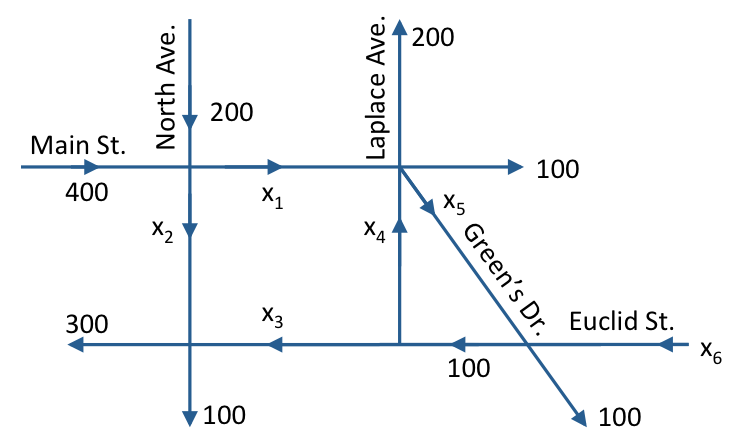
\includegraphics[width=0.8\textwidth]{Traffic.png}
  \end{center}
  \vspace{-20pt}
\end{figure}
Set up a linear system of equations that could be used to determine all of the $x$'s, and find the value of $x_6$ so that the system has exactly one solution. Assume that the total number of cars in this area of the city remains constant throughout Saturday afternoons. \textit{Hint: you shouldn't need to use a computer or row reduction to find $x_6$}.
% ~~~~~~~~~~~~~~~~~~~~~~~~~~~~~~~~~~~~~~~~~~~~~~~~~~~~~~~~~~~~~~~~~~~~~~~~~~~~~~~~~
\item % NAVIER STOKES
When a particle moves through a liquid in a region of $\R^3$, it traces out a path $C$ described by $x=x(t), y=y(t), z=z(t)$, where $t$ represents time. If $\rho=\rho(x,y,z,t)=\rho\big(x(t),y(t),z(t),t\big)$ is the density of the fluid at time $t$, show that, along $C$,
\begin{align*}
  \frac{d\rho}{dt} &= \frac{\partial \rho}{\partial t} + \nabla \rho \cdot \MB{r}'(t),
\end{align*}
where $\MB{r} = x\MB{i}+y\MB{j}+z\MB{k}$.
% ~~~~~~~~~~~~~~~~~~~~~~~~~~~~~~~~~~~~~~~~~~~~~~~~~~~~~~~~~~~~~~~~~~~~~~~~~~~~~~~~~
\item % AREA OF A TRIANGLE
Find the area of the triangle with vertices $(0,0,0)$, $(1,0,0)$, and $(0,1,1)$ using a double integral. \textit{Hint: you may want to check your answer by calculating the area another way (for example, by using a cross product)}.

% ~~~~~~~~~~~~~~~~~~~~~~~~~~~~~~~~~~~~~~~~~~~~~~~~~~~~~~~~~~~~~~~~~~~~~~~~~~~~~~~~~
\item % CHAIN RULE
Let $f=-\frac{x^2}{2}+y^3$, and $\phi$ be a differentiable function of $x$, so that $\phi = \phi(x)$. Suppose also that $f(x,\phi(x))=\frac{1}{2}$ for all $x$. Find $\phi'(1)$, and do not leave your answer in terms of $\phi$. \rednote{We probably want to move this question back to a written assignment}
% ~~~~~~~~~~~~~~~~~~~~~~~~~~~~~~~~~~~~~~~~~~~~~~~~~~~~~~~~~~~~~~~~~~~~~~~~~~~~~~~~~
\item % LINEAR PROGRAMMING
Suppose that we wish to minimize a function of the form $f=Ax+By$, where $A$ and $B$ are positive constants, subject to the constraint that we may only consider points in the region $D$ that describes a polygon in the $xy$-plane. Let the region $D$ be the 
\BEN
\item By considering level sets of $f(x,y)$, show that $f$ is minimized at one or more vertices of region $D$. Use $\nabla f$ in your explanation. 
\item For what values of $A$ and $B$ does the minimum values of $f$ have two minima? 
\EEN
% ~~~~~~~~~~~~~~~~~~~~~~~~~~~~~~~~~~~~~~~~~~~~~~~~~~~~~~~~~~~~~~~~~~~~~~~~~~~~~~~~~
\item % CONSTRUCT A FUNCTION WITH CRITICAL POINTS
Provide an example of a function of two variables, $f(x,y)$, that has the following properties. 
\begin{itemize}
  \item $f(x,y)$ has no more than four critical points on $\R^2$.
  \item $f(x,y)$ has a maximum at the point $(a,0)$, and a minimum at the point $(0,b)$, where $a<0$ and $b>0$.
  \item $f(x,y)$ is continuous everywhere on $\R^2$.
\end{itemize}
Show that your function satisfies the above properties. 

% ~~~~~~~~~~~~~~~~~~~~~~~~~~~~~~~~~~~~~~~~~~~~~~~~~~~~~~~~~~~~~~~~~~~~~~~~~~~~~~~~~
\item % 
Calculate the volume of ...
% ~~~~~~~~~~~~~~~~~~~~~~~~~~~~~~~~~~~~~~~~~~~~~~~~~~~~~~~~~~~~~~~~~~~~~~~~~~~~~~~~~
\item % 

% ~~~~~~~~~~~~~~~~~~~~~~~~~~~~~~~~~~~~~~~~~~~~~~~~~~~~~~~~~~~~~~~~~~~~~~~~~~~~~~~~~
\item %

% ~~~~~~~~~~~~~~~~~~~~~~~~~~~~~~~~~~~~~~~~~~~~~~~~~~~~~~~~~~~~~~~~~~~~~~~~~~~~~~~
\item In one paragraph, please describe the importance of interdisciplinary engineering today. Please use examples of interdisciplinary fields and works. Your paragraph should not exceed $X$ words, where $X$ is a number that your instructor will provide. 
% ~~~~~~~~~~~~~~~~~~~~~~~~~~~~~~~~~~~~~~~~~~~~~~~~~~~~~~~~~~~~~~~~~~~~~~~~~~~~~~~~~
\end{enumerate} % END OF QUESTIONS
% ~~~~~~~~~~~~~~~~~~~~~~~~~~~~~~~~~~~~~~~~~~~~~~~~~~~~~~~~~~~~~~~~~~~~~~~~~~~~~~~~~
% ~~~~~~~~~~~~~~~~~~~~~~~~~~~~~~~~~~~~~~~~~~~~~~~~~~~~~~~~~~~~~~~~~~~~~~~~~~~~~~~~~
% ~~~~~~~~~~~~~~~~~~~~~~~~~~~~~~~~~~~~~~~~~~~~~~~~~~~~~~~~~~~~~~~~~~~~~~~~~~~~~~~~~
% SOLUTIONS
\newpage
\section*{Solutions}

\begin{enumerate}
% ~~~~~~~~~~~~~~~~~~~~~~~~~~~~~~~~~~~~~~~~~~~~~~~~~~~~~~~~~~~~~~~~~~~~~~~~~~~~~~~~~
\item % TRAFFIC
For any intersection, the number of cars leaving the intersection must equal the number of cars entering the intersection. For the intersection of North and Main,
\begin{align*}
 100+400 = x_1+x_2.
\end{align*}
The other intersections give us the equations:
\begin{align*}
 x_1+x_4 &=200+x_5+100 \quad \text{ (at Laplace, Green's, Main)}\\
 x_2+x_3 &=300+100 \quad \text{ (at Euclid and North)}\\
 x_3+x_4 &=100 \quad \text{ (at Euclid and Laplace)}\\
 100+x_5 &=100+x_6 \quad \text{ (at Green's and Euclid)}
\end{align*}
We can collect these equations into the system
\begin{align*}
\BM 
1 & 1 & 0 & 0 & 0 & 0 \\
1 & 0 & 0 & 1 &-1 & 0 \\
0 & 1 & 1 & 0 & 0 & 0 \\
0 & 0 & 1 & 1 & 0 & 0 \\
0 & 0 & 0 & 0 & 1 & -1
\EM 
\BM x_1 \\ x_2 \\ x_3 \\ x_4 \\ x_5 \\ x_6 \EM
= \BM 500 \\ 300 \\ 400 \\100\\100\EM
\end{align*}
If the total number of cars remains constant, the number of cars entering the downtown area must equal the number of cars leaving the downtown area. Mathematically, this means:
\begin{align*}
  \text{Number of cars entering downtown} &= \text{number of cars leaving downtown} \\
  x_6 + 400 + 200 &= 100 + 100 + 100 + 300 \\
  x_6 &= 0
\end{align*}
A more tedious, but acceptable method would be to row-reduce the above system and find a value of $x_6$ such that the system is consistent.


% ~~~~~~~~~~~~~~~~~~~~~~~~~~~~~~~~~~~~~~~~~~~~~~~~~~~~~~~~~~~~~~~~~~~~~~~~~~~~~~~~~
\item % NAVIER STOKES
Applying the chain rule:
\begin{align*}
  \frac{d\rho}{dt} &= \frac{\partial \rho}{\partial t} + \frac{\partial \rho}{\partial x} \pxt + \frac{\partial \rho}{\partial y} \pyt +\frac{\partial \rho}{\partial z} \pzt \\
  &= \frac{\partial \rho}{\partial t} + \BM \frac{\partial \rho}{\partial x}  \\ \\  \frac{\partial \rho}{\partial y} \\ \\ \frac{\partial \rho}{\partial z}\EM \cdot \BM \pxt \\\\ \pyt \\\\ \pzt \EM \\
    &= \frac{\partial \rho}{\partial t} + \nabla \rho \cdot \MB{r}'(t). 
\end{align*}

% ~~~~~~~~~~~~~~~~~~~~~~~~~~~~~~~~~~~~~~~~~~~~~~~~~~~~~~~~~~~~~~~~~~~~~~~~~~~~~~~~~
\item % AREA OF A TRIANGLE
The length of the sides of the right-angled triangle whose area we need can be determined with the distance formula. The triangle has sides of length $\sqrt{2}$, $1$, and the length of its hypotenuse is $\sqrt{3}$. Using these lengths, we can construct a triangle in $\R^2$ whose area is the area of the triangle we were given. The hypotenuse can be described by the line $y=-\sqrt{2}(x-1)$. The double integral that gives us the area is 
\begin{align*}
  \mathop{\int_0^1 \!\! \int_{0}^{-\sqrt{2}(x-1)}} dydx &= 
  \int_0^1 \Big(-\sqrt{2}(x-1)\Big)dx \\
  &= -\sqrt{2} \int_0^1 (x-1) dx \\
  &= -\sqrt{2} \Big(\frac{x^2}{2}-x\Big)\Big|_0^1 \\
  &= -\sqrt{2}\Big(\frac{-1}{2}\Big) \\
  &= \frac{\sqrt{2}}{2}.
\end{align*}
% ~~~~~~~~~~~~~~~~~~~~~~~~~~~~~~~~~~~~~~~~~~~~~~~~~~~~~~~~~~~~~~~~~~~~~~~~~~~~~~~~~
\item % CHAIN RULE
Differentiating $f(x,\phi(x))=\frac{1}{2}$ with respect to $x$ gives us 
\begin{align*}
  \px f(x,\phi) = 0 &= \px \Big(-\frac{x^2}{2} + \big(\phi(x)\big)^3\Big)\\
  &= -x + 3\big(\phi(x)\big)^2\phi'(x)
\end{align*}
At $x=1$ this becomes
\begin{align*}
  0 &= -1 + 3\big(\phi(1)\big)^2\phi'(1)\\
  \phi'(1) &=\frac{1}{3\big(\phi(1)\big)^2}
\end{align*}
But $f(x,\phi(x))=\frac{1}{2}$, and $f=-\frac{x^2}{2}+y^3$, so at $x=1$,
\begin{align*}
  f(x,\phi) = \frac{1}{2} 
  &= \Big(-\frac{x^2}{2} + \big(\phi(x)\big)^3\Big)\\
  &= \Big(-\frac{1^2}{2} + \big(\phi(1)\big)^3\Big)\\
  \big(\phi(1)\big)^3 &= 1\\
  \phi(1) &= 1
\end{align*}
Finally,
\begin{align*}
  \phi'(1) &= \frac{1}{3}.
\end{align*}
% ~~~~~~~~~~~~~~~~~~~~~~~~~~~~~~~~~~~~~~~~~~~~~~~~~~~~~~~~~~~~~~~~~~~~~~~~~~~~~~~~~
\item % LAGRANGE
To ...
% ~~~~~~~~~~~~~~~~~~~~~~~~~~~~~~~~~~~~~~~~~~~~~~~~~~~~~~~~~~~~~~~~~~~~~~~~~~~~~~~~~
\item % CONSTRUCT A FUNCTION WITH CRITICAL POINTS
We need a function with critical points when $x=0$ and when $x=a$. Thus, $\px f$ must be zero at these points. One example of such a function is
\begin{align*}
  \px f(x,y) = x(x-a),
\end{align*}
or, integrating with respect to $x$, we obtain
\begin{align*}
  f(x,y) = \int (x^2-ax)dx + g(y) = \frac{x^3}{3}-a\frac{x^2}{2}+g(y).
\end{align*}
Our function must also have critical points when $y=0$ and when $y=b$. This gives us constraints that we can use to find $g$. Differentiating with respect to $y$:
\begin{align*}
  \py f(x,y) = g'(y).
\end{align*}
Setting $g'(y)=y(y-b)$, gives us, after integration
\begin{align*}
  f(x,y) = \frac{x^3}{3}+ \frac{y^3}{3}-a\frac{x^2}{2}-b\frac{y^2}{2}.
\end{align*}
We need our function to have a maximum at $(a,0)$, which requires that $D>0$ and $f_{xx}<0$ at $(a,0)$.
\begin{align*}
  D &= \Big(f_{xx}f_{yy}-f_{xy}\Big)\Big|_{(a,0)} \\
  &= (2x-a)(2y-b)\Big|_{(a,0)} \\
  &= -ab.
\end{align*}
Because $a<0$, and $b>0$, $D$ is positive. And because $f_{xx}(a,0)=a$, $(a,0)$ is a maximum. 

Likewise, we need our function to have a min at $(0,b)$, which requires that $D>0$ and $f_{xx}>0$ at $(0,b)$.
\begin{align*}
  D &= \Big(f_{xx}f_{yy}-f_{xy}\Big)\Big|_{(0,b)} \\
  &= (2x-a)(2y-b)\Big|_{(0,b)} \\
  &= -ab.
\end{align*}
Because $a<0$, and $b>0$, $D$ is positive. And because $f_{xx}(0,b)=-a$, $(0,b)$ is a maximum. 

Also note that our $f$ has only four critical points, at $(0,0), (a,0), (0,b), (a,b)$, and because $f$ is a polynomial, it is continuous everywhere on $\R^2$. 

\end{enumerate}

\end{document}
